% Figure: answering one OuMv request with switches (Lemma~\ref{lem:round}).
% Requires only tikz. Same colors as the gadget figure: rows vermillion, columns blue.
\begin{figure}[t]
\centering
\providecommand\Description[2][]{}%
\Description{A five-by-five zero-one matrix with two rows shaded orange and two columns shaded blue; their four intersection cells are darker. Beside it a legend of switch states (hollow or filled row cycle, filled or hollow tether) and the identity relating beta two to the rank of the active submatrix.}
\definecolor{omRow}{HTML}{D55E00}%
\definecolor{omCol}{HTML}{0072B2}%
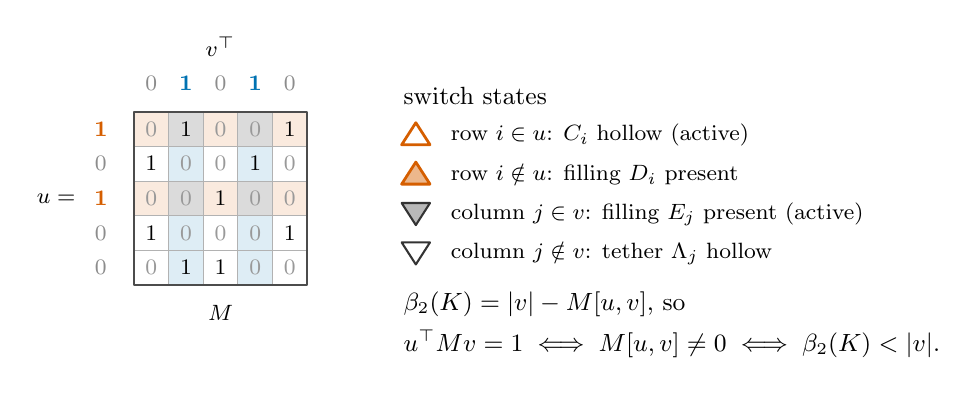
\begin{tikzpicture}[x=1cm,y=1cm,line join=round,font=\footnotesize]
  \def\s{0.44}
  % M with rows i = 1..5 (top to bottom) and columns j = 1..5
  \def\M{{{0,1,0,0,1},{1,0,0,1,0},{0,0,1,0,0},{1,0,0,0,1},{0,1,1,0,0}}}
  % highlight active rows (supp u = {1,3}) and active columns (supp v = {2,4})
  \foreach \i in {1,3} \fill[omRow!13] (0,{-\i*\s}) rectangle (5*\s,{-(\i-1)*\s});
  \foreach \j in {2,4} \fill[omCol!13] ({(\j-1)*\s},0) rectangle ({\j*\s},-5*\s);
  \foreach \i in {1,3} \foreach \j in {2,4} \fill[black!14] ({(\j-1)*\s},{-\i*\s}) rectangle ({\j*\s},{-(\i-1)*\s});
  \draw[black!30,line width=0.3pt] (0,0) grid[step=\s] (5*\s,-5*\s);
  \draw[black!70,line width=0.6pt] (0,0) rectangle (5*\s,-5*\s);
  \foreach \i in {1,...,5} \foreach \j in {1,...,5} {
    \pgfmathtruncatemacro{\e}{\M[\i-1][\j-1]}
    \ifnum\e=1 \node[inner sep=0pt,text=black] at ({(\j-0.5)*\s},{-(\i-0.5)*\s}) {$1$};
    \else \node[inner sep=0pt,text=black!40] at ({(\j-0.5)*\s},{-(\i-0.5)*\s}) {$0$}; \fi
  }
  % u and v
  \foreach \i/\e in {1/1,2/0,3/1,4/0,5/0} {
    \ifnum\e=1 \node[inner sep=0pt,text=omRow] at (-0.42,{-(\i-0.5)*\s}) {$\mathbf{1}$};
    \else \node[inner sep=0pt,text=black!45] at (-0.42,{-(\i-0.5)*\s}) {$0$}; \fi}
  \foreach \j/\e in {1/0,2/1,3/0,4/1,5/0} {
    \ifnum\e=1 \node[inner sep=0pt,text=omCol] at ({(\j-0.5)*\s},0.36) {$\mathbf{1}$};
    \else \node[inner sep=0pt,text=black!45] at ({(\j-0.5)*\s},0.36) {$0$}; \fi}
  \node[anchor=east] at (-0.62,{-2.5*\s}) {$u=$};
  \node[anchor=south] at ({2.5*\s},0.58) {$v^{\top}$};
  \node at ({2.5*\s},{-5*\s-0.35}) {$M$};
  % the switch states
  \begin{scope}[shift={(3.3,0.2)}]
    \node[anchor=west,font=\small] at (0,0) {switch states};
    \path[draw=omRow,line width=1pt,fill=white] (0.1,-0.62) -- (0.46,-0.62) -- (0.28,-0.34) -- cycle;
    \node[anchor=west] at (0.6,-0.5) {row $i\in\supp u$: $C_i$ hollow (active)};
    \path[draw=omRow,line width=1pt,fill=omRow!45] (0.1,-1.12) -- (0.46,-1.12) -- (0.28,-0.84) -- cycle;
    \node[anchor=west] at (0.6,-1.0) {row $i\notin\supp u$: filling $D_i$ present};
    \path[draw=black!80,line width=0.75pt,fill=black!28] (0.1,-1.36) -- (0.46,-1.36) -- (0.28,-1.64) -- cycle;
    \node[anchor=west] at (0.6,-1.5) {column $j\in\supp v$: filling $E_j$ present (active)};
    \path[draw=black!80,line width=0.75pt,fill=white] (0.1,-1.86) -- (0.46,-1.86) -- (0.28,-2.14) -- cycle;
    \node[anchor=west] at (0.6,-2.0) {column $j\notin\supp v$: tether $\Lambda_j$ hollow};
    \node[anchor=west,font=\small] at (0,-2.65) {$\beta_2(K)=|\supp v|-\rk M[\supp u,\supp v]$, so};
    \node[anchor=west,font=\small] at (0,-3.15) {$u^{\top}Mv=1 \iff M[\supp u,\supp v]\neq0 \iff \beta_2(K)<|\supp v|$.};
  \end{scope}
\end{tikzpicture}
\caption{Answering one \OuMv\ request $(u,v)$ with the gadget $\Kswitch{M}{R}{J}$; see Lemma~\ref{lem:round}(i).
Exactly the rows in $R=\supp u$ and the columns in $J=\supp v$ are switched on, so the active part of~$M$ is the submatrix $M[R,J]$ (dark cells).
Here $M[R,J]$ contains a~$1$, so $\rk M[R,J]=1$, $\beta_2=|J|-1<|J|$, and the Boolean product $u^{\top}Mv$ is~$1$.
Moving from one request to the next takes at most $2\ell$ switches, each of which inserts or deletes a single triangle.}
\label{fig:oumv}
\end{figure}
